\chapter{\textbf{Технологический раздел}}

\hfill

В соответствии с выбранной задачей -- визуализацией взрыва. Необходимо выбрать средства реализации, создать интерфейс и структуры программного обеспечения, описать ограничения и порядок работы программы. 

\section{\textbf{Выбор и обоснование языка программирования }}

Для выполнения проекта был выбран язык программирования C++/QT.

C++ -- компилируемый, статически типизированный язык программирования общего назначения \cite{c++}. 

C++ сочетает свойства высокоуровневого и низкоуровневого языка. В сравнении с его предшественником, языком C, присутствует поддержка объектно-ориентированного программирования.

Являясь одним из самых популярных языков программирования, C++ широко используется для разработки программного обеспечения \cite{usingc++}. 

Qt -- кроссплатформенная библиотека разработки GUI на С++ \cite{qt}.

Библиотека Qt является безусловным лидером среди имеющихся средств разработки кроссплатформенных приложений на языке C++. Qt – полностью объектно-ориентированная библиотека.

Все элементы в окне программы, кнопки, переключатели - это отдельные виджеты. Именно виджеты являются основой построения графических интерфейсов. С точки зрения программы, они воспринимают все
события и генерируют сигналы, которые в свою очередь вызывают слоты – специальные функции, реагирующие на различные события в окне. 

Qt прекрасно документирована, благодаря чему всегда можно найти о ней любую интересующую информацию.

Для написания программного кода использовался Qt Creator 4.8.1. Основная задача Qt Creator -- упростить разработку приложения с помощью фреймворка Qt на различных платформах.

\section{\textbf{Интерфейс пользователя }}

Взаимодействие пользователя с приложением осуществляется через интерфейс, представленный на рисунке \ref{img:interface}. 

\begin{figure}[H]
	\centering
	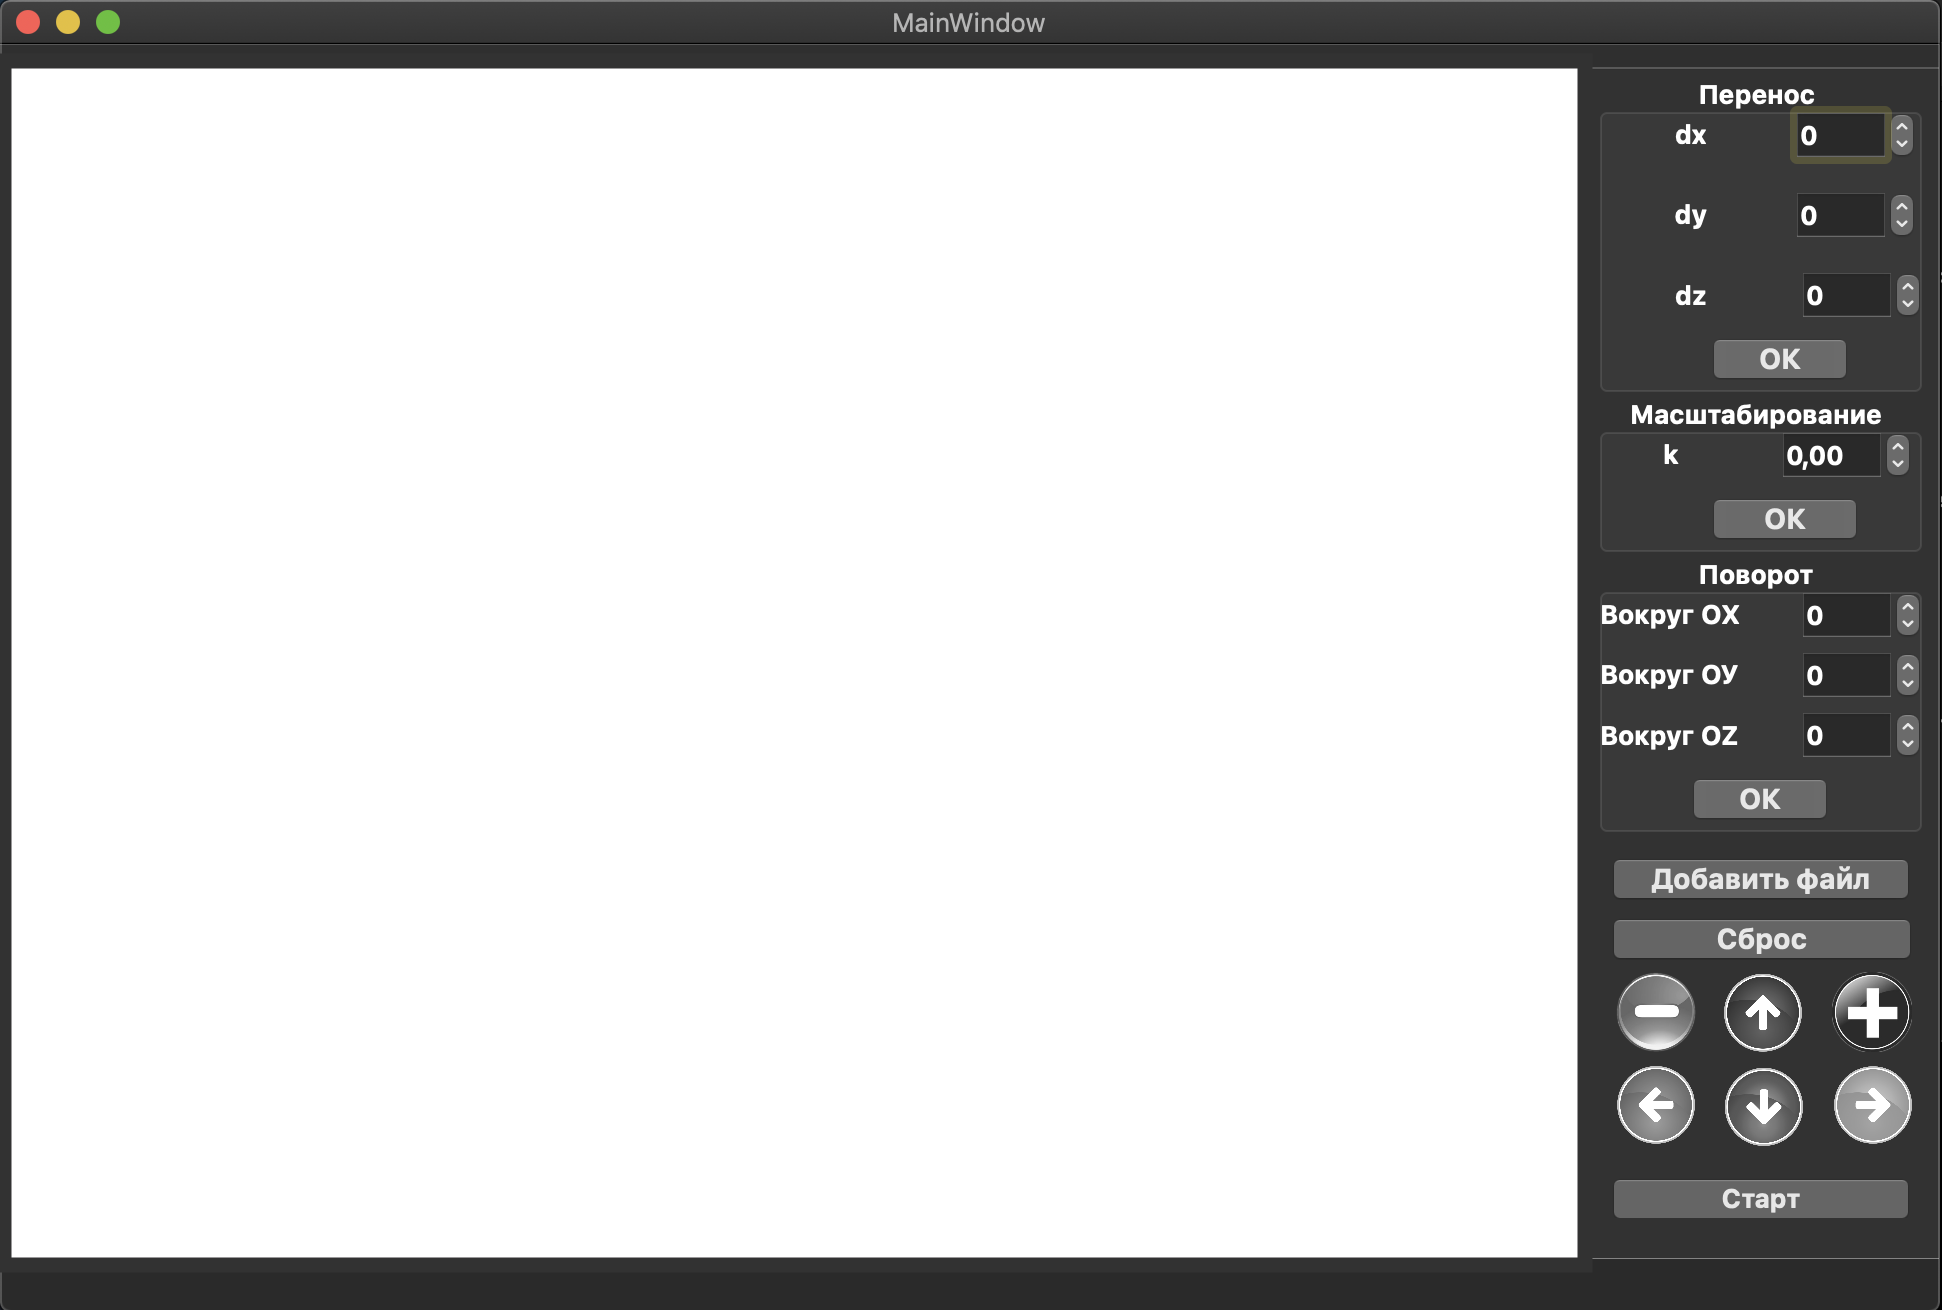
\includegraphics[scale=0.4]{interface}
	\caption{Интерфейс пользователя}
	\label{img:interface}
\end{figure}

\begin{enumerate}
	\item Доступны поля для ввода данных, при желании менять расположение и вид объектов. 
	\item Кнопки ($\to, \leftarrow, \uparrow, \downarrow, +, -$) предназначены для взаимодействия с камерой. 
	\item Кнопка  <<Сброс>> -- сбрасывает все настройки в начальное состояние. 
	\item Кнопка <<Добавить файл>> -- для загрузки данных. 
	\item Кнопка <<GO>> - запускает приложение.   
\end{enumerate}

\section{\textbf{Хранение и обмен данными в системе }}


\section{\textbf{Разработка программы и тестовых примеров }}


\section{\textbf{Требования к аппаратуре }}


\section{\textbf{Требования к программному обеспечению }}


\section{\textbf{Порядок работы }}


\section{\textbf{Обращение к программе }}


\section{\textbf{Входные и выходные данные }}


\section{\textbf{Сообщения  системы }}

